
\section{Ejercicio 2}


\subsection{Experimentación}
El loteEj2.tsk contiene lo pedido por enunciado.

TaskCPU 100  

TaskConsola 20 2 4

TaskConsola 25 2 4

Veamos que tiene un uso de 100 de cpu que es del algoritmo complejo, un TaskConsola que es para la canción que realiza 20 llamadas bloqueantes y el otro de 25 para navegar por
internet. Las llamadas bloqueantes son entre 2 y 4.

\begin{figure}[H]
  \centering
    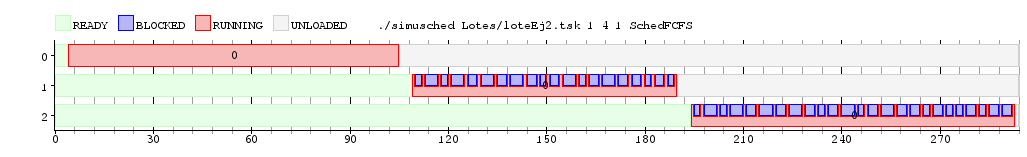
\includegraphics[width=1.1\textwidth]{imagenes/Ej2Experimento1core.png}
  \caption{loteEj2.tsk con FCFS y coste cambio de contexto de 4 ciclos con 1 núcleo}
\end{figure}

\begin{tabular}{l | r }
  Proceso & Latencia\\
  \hline
  CPU & 4\\
  Canción favorita & 108\\
  Navegar por Internet & 194\\
\end{tabular}

\begin{figure}[H]
  \centering
    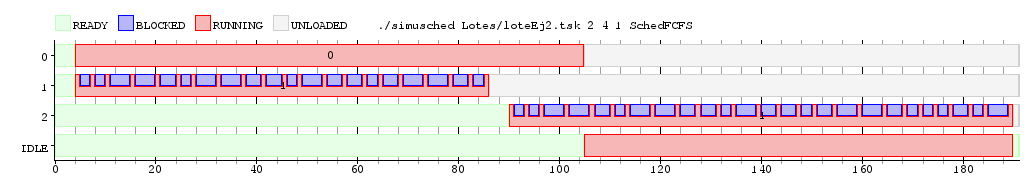
\includegraphics[width=1.1\textwidth]{imagenes/Ej2Experimento2core.png}
  \caption{loteEj2.tsk con FCFS y coste cambio de contexto de 4 ciclos con 2 núcleo}
\end{figure}

\begin{tabular}{l | r }
  Proceso & Latencia\\
  \hline
  CPU & 4\\
  Canción favorita & 4\\
  Navegar por Internet & 91\\
\end{tabular}

Hay que aclarar que las latencias podrían variar ya que TaskConsola genera las llamadas bloqueantes con un tamaño aleatorio entre 2 y 4. Podemos ver que en el primer caso se
debe esperar hasta que el algoritmo complejo termine para poder escuchar musica y , a su vez, que esto termine para poder navegar por internet. En el segundo caso, vemos que 
se puede ejecutar el algoritmo complejo y escuchar la canción al mismo tiempo, pero se debe terminar la canción para poder navegar por internet. Este último es mejor porque
la canción y navegar por internet tienen latencias menores. 

Rolando va a tener muchos problemas para ejecutar esto con un solo núcleo ya que mientras se este ejecutando el cpu no se podrá hacer ninguna de las otras cosas, que es lo que él
pretende. Una buena solución sería tener 3 núcleos para que las tres cosas se puedan hacer al mismo tiempo. Otra sería usar Round-Robin para poder ir alternando los procesos y 
que no tenga que esperar que uno termine para poder ir ejecutando los otros.